\section{Structures de données}

    \subsection{XML}
        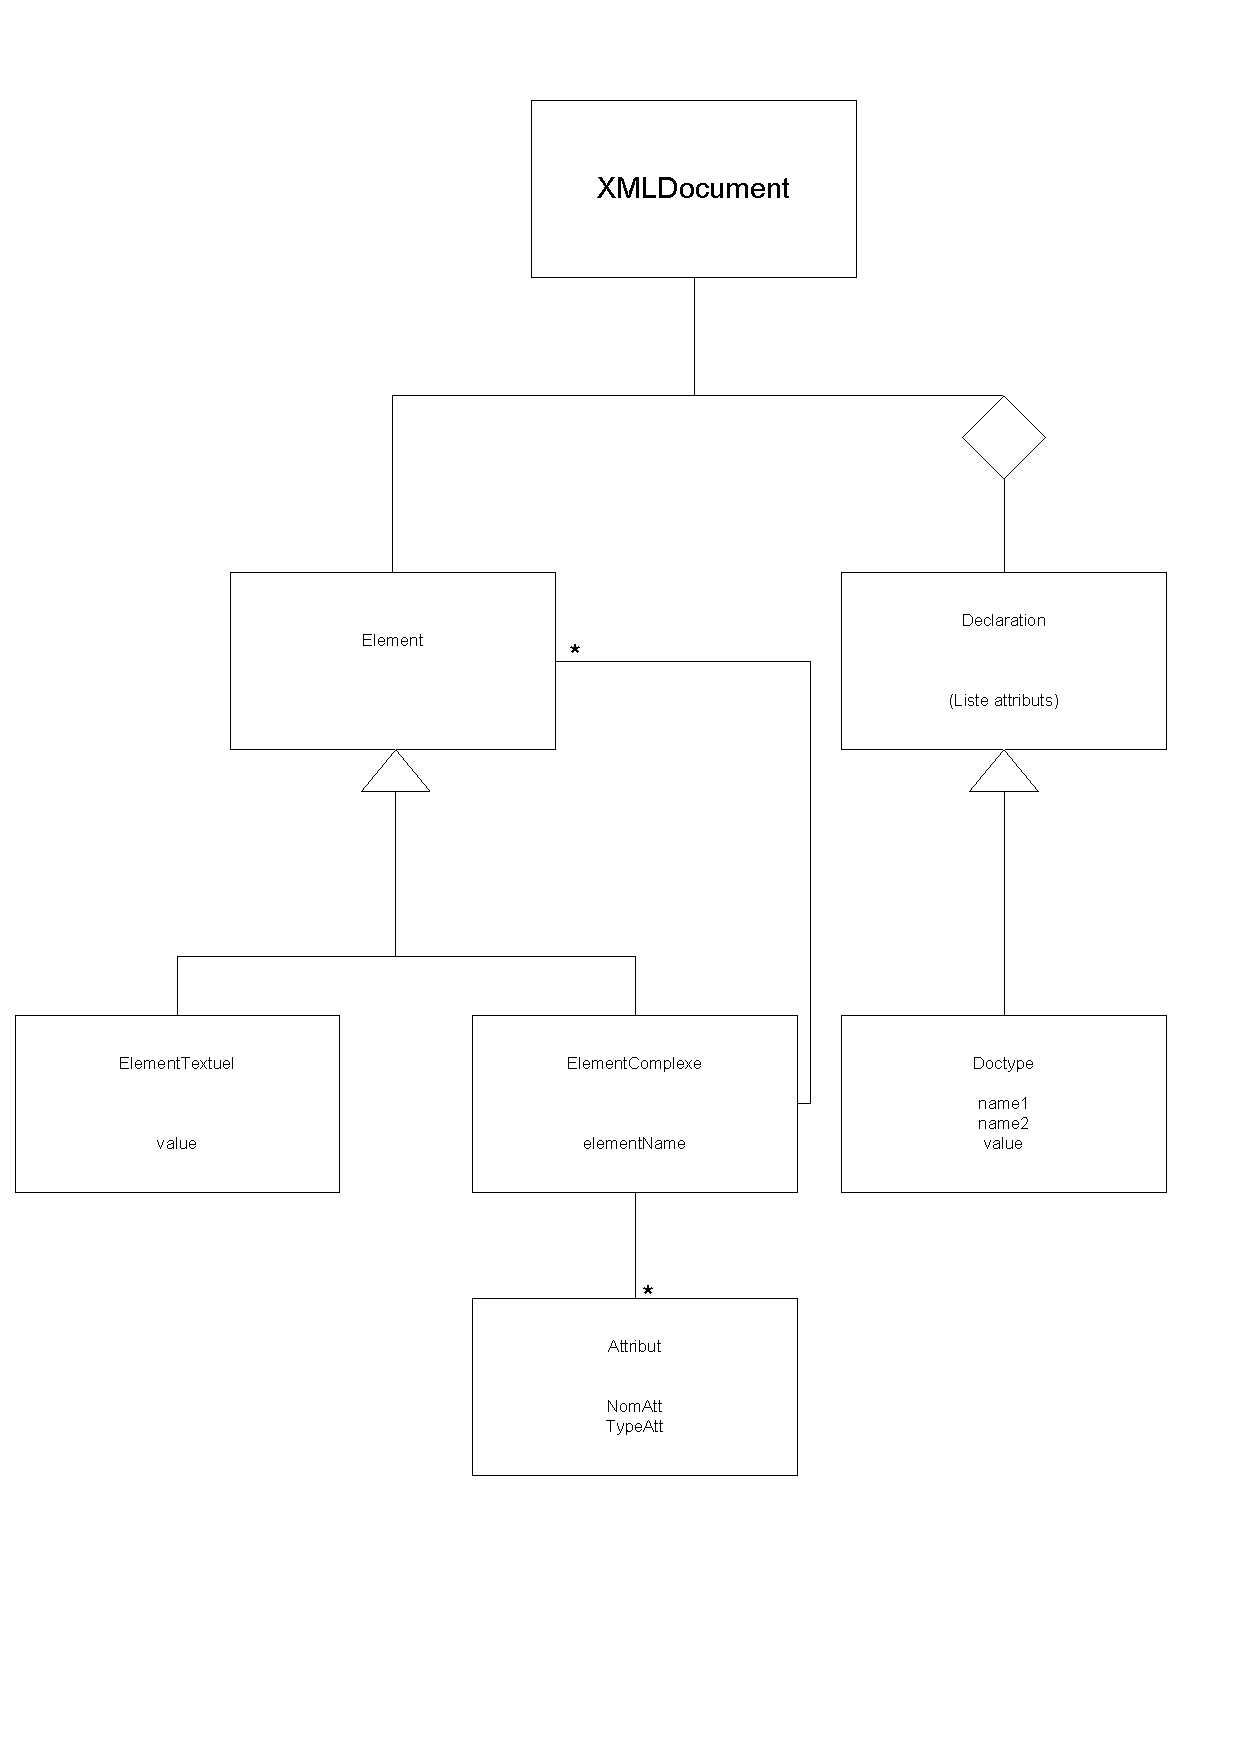
\includegraphics[width=0.7\textwidth]{img/ClassesXML.pdf}\\
        La structure de donnée généré pendant la lecture du XML
        
    \subsection{DTD}
        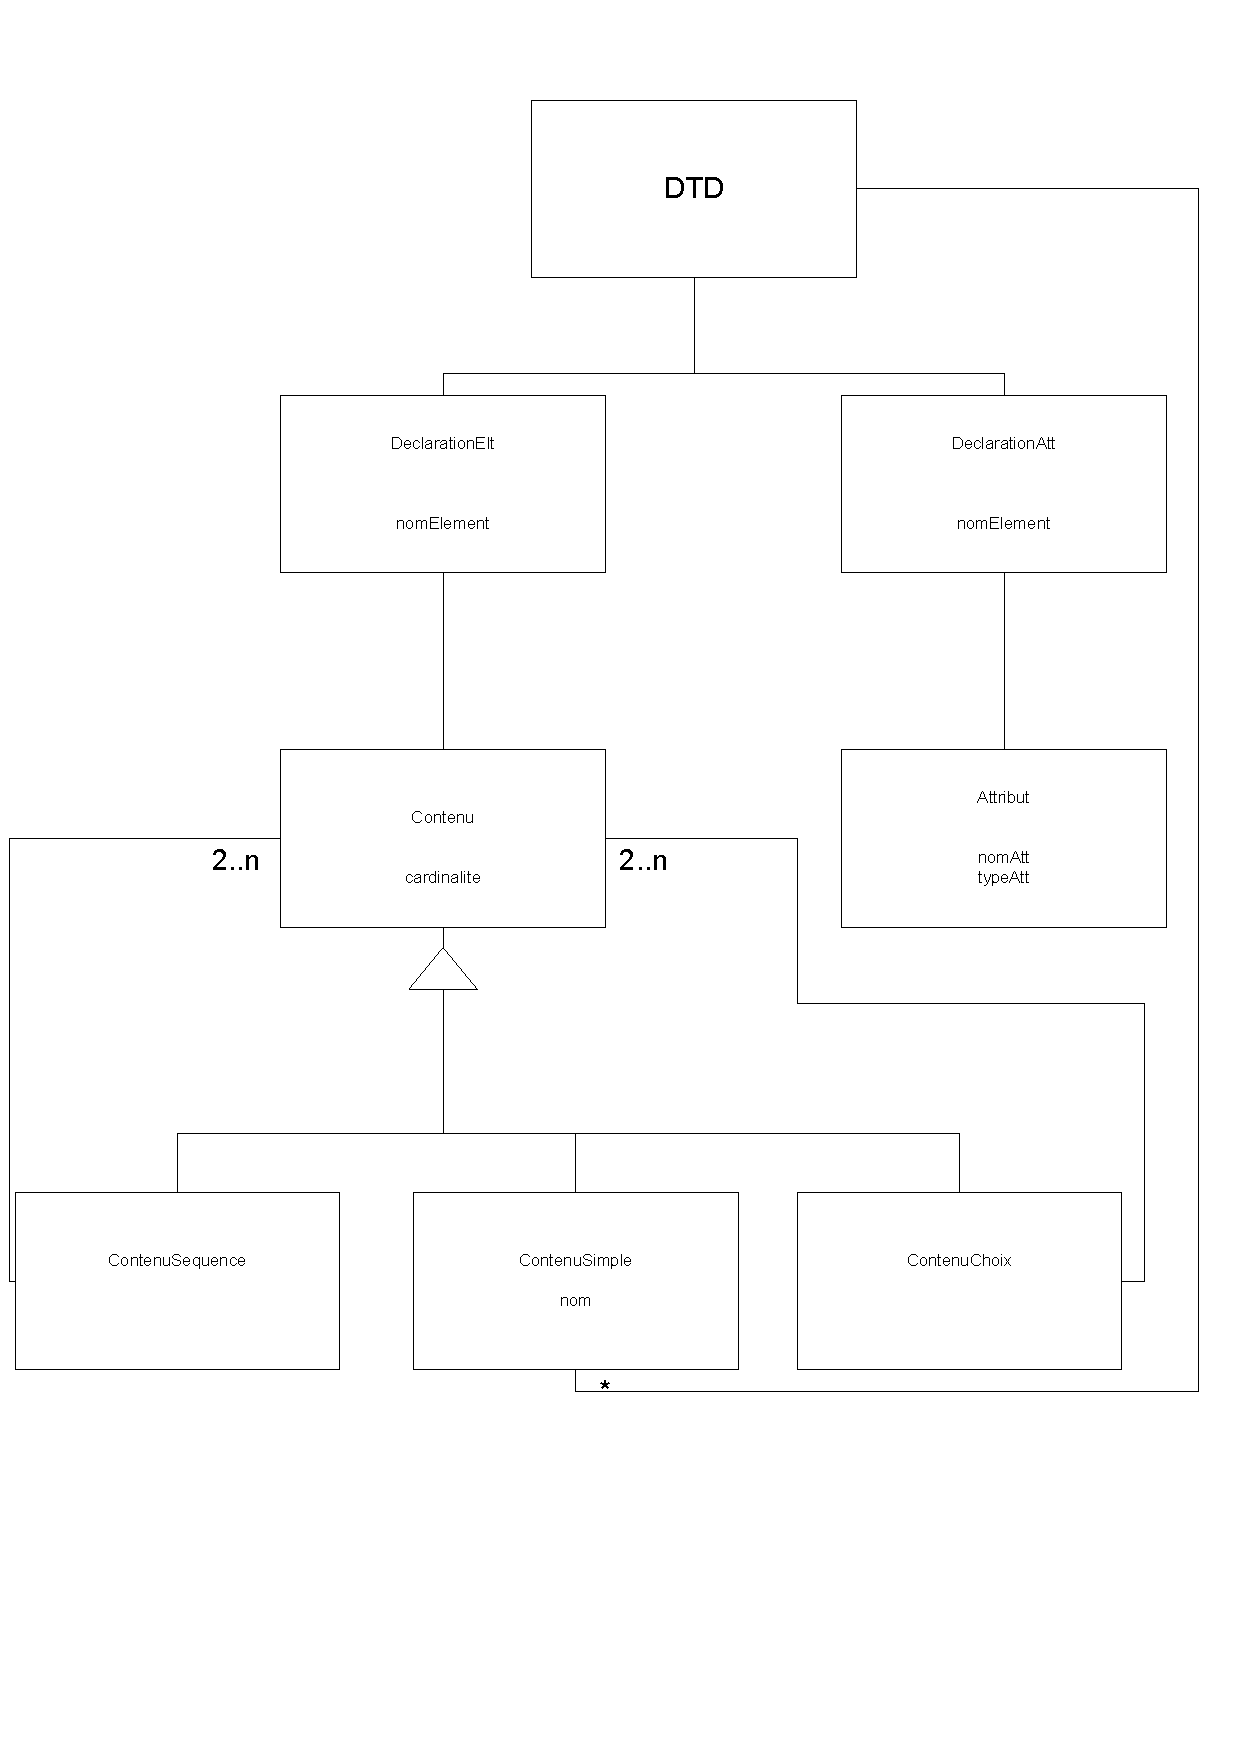
\includegraphics[width=0.7\textwidth]{img/ClassesDTD.pdf}\\
        La structure de donnée généré pendant la lecture de la DTD
        
\section{Algorithmes}

    \subsection{Validation}
	
	validateXML(XML xml, DTD dtd){
		String exp =transformXML(xml) // transfomer le fichier XML en 1 expression a valider
		String pattern = transformDTD(dtd) // transformer le fichier DTD en pattern 
		bool resultat = match(exp, pattern) // valider 		
	}

	transformDTD(DTD dtd){
		RETOURNER tranformDeclarationElement(dtd.racine) //on commencer par l'element racine
	}

	tranformDeclarationElement(DeclarationElement decEle) // transformer recursivement 
	{
		String return;
		SI (decEle est textuel) //si element textuel (pas de fils)
		{
			result="<"+decEle.nom+decATTLIST">decText"</"+decEle.nom+">
		}
		SINON
		{
			result ="(<"+decEle.nom+decATTLIST">";
			pour chaque element fils filsEle{
				SI PAS CONTRAINTE CARDINALITE:
					result += tranformDeclarationElement(filsEle);
				SINON
					result += "(" tranformDeclarationElement(filsEle)+cadinalite(filsEle)+")";
			}	
		}
	}

        
    \subsection{Transformation}
        %TODO ici l'algo fait par Baptiste
